\documentclass{article}

% if you need to pass options to natbib, use, e.g.:
%     \PassOptionsToPackage{numbers, compress}{natbib}
% before loading neurips_2019

% ready for submission
% \usepackage{neurips_2019}

% to compile a preprint version, e.g., for submission to arXiv, add add the
% [preprint] option:
    \usepackage[preprint]{neurips_2019}

% to compile a camera-ready version, add the [final] option, e.g.:
    %  \usepackage[final]{neurips_2019}

% to avoid loading the natbib package, add option nonatbib:
%     \usepackage[nonatbib]{neurips_2019}

\usepackage[utf8]{inputenc} % allow utf-8 input
\usepackage[T1]{fontenc}    % use 8-bit T1 fonts
\usepackage{hyperref}       % hyperlinks
\usepackage{url}            % simple URL typesetting
\usepackage{booktabs}       % professional-quality tables
\usepackage{amsfonts}       % blackboard math symbols
\usepackage{nicefrac}       % compact symbols for 1/2, etc.
\usepackage{microtype}      % microtypography
\usepackage{graphicx,graphics,subcaption}
\usepackage{graphicx,graphics,color}


\usepackage{mathtools}

\newtheorem{theorem}{Theorem}[section]
\newtheorem{corollary}{Corollary}[theorem]
\newtheorem{lemma}[theorem]{Lemma}
\newtheorem{definition}[theorem]{Definition}
\newtheorem{appendx}{Appendix}


\title{A comprehensive study on binary optimizer and its applicability}

% The \author macro works with any number of authors. There are two commands
% used to separate the names and addresses of multiple authors: \And and \AND.
%
% Using \And between authors leaves it to LaTeX to determine where to break the
% lines. Using \AND forces a line break at that point. So, if LaTeX puts 3 of 4
% authors names on the first line, and the last on the second line, try using
% \AND instead of \And before the third author name.

\makeatletter
\newcommand{\printfnsymbol}[1]{%
  \textsuperscript{\@fnsymbol{#1}}%
}
\makeatother
\author{%
  Nancy Nayak\thanks{equal contribution has been made by the authors}, Vishnu Raj\printfnsymbol{1}, Sheetal Kalyani \\
  Department of Electrical Engineering \\
  Indian Institute of Technology, Madras\\
  Chennai, India 600036 \\
  \texttt{\{ee17d408@smail, ee14d213@ee, skalyani@ee\}.iitm.ac.in} \\
}




\begin{document}

\maketitle
    \begin{abstract}
Binarized Neural Networks are paving a way towards the deployment of deep neural networks with less memory and computation. In this report, we present a detailed study on the paper titled "Latent Weights Do Not Exist: Rethinking Binarized Neural Network Optimization" by \cite{helwegen2019latent} which proposes a new optimization method for training BNN called BOP. We first investigate the effect of using latent weights in BNN for analyzing prediction performance in terms of accuracy. Next, a comprehensive ablation study on hyperparameters is provided. Finally, we explore the usability of BNN in denoising autoencoders. Code for all our experiments are available at  \url{https://github.com/nancy-nayak/rethinking-bnn/}
\end{abstract}
    \section{Introduction}
In the era of Artificial Intelligence, deep learning methods are finding themselves useful in a variety of tasks. This is not only limited to image or speech processing using supervised learning, game playing using reinforcement learning but to more complex tasks ranging from self driving car to smart personal assistants to autonomous drones helping with household work. The main challenge of using deep learning in computationally complex tasks is that it requires a big complex network which in turn requires huge memory to save its parameters and high computational power. These big networks are often trained with one or many power hungry GPUs. However, in order to enter a mass deployment of solutions, methods that can run low power devices are desirable. In order to satisfy the need of good performance of these networks but deployed with less resources in terms of memory and compute, \cite{courbariaux2015binaryconnect} proposed Binaryconnect in which the learnt parameters are limited $+1$ or $-1$. Later \cite{courbariaux2016binarized} introduced  binary neural networks (BNN) where activation also is a binarization function. The main problem of training BNN is that the gradient of binarization function is almost zero everywhere. This was mitigated by utilizing a special kind of function called straight through estimator (STE) \cite{hinton_coursera} . To train these neural networks with binary weights, a popular choice is to use Adam optimizer \cite{kingma2014adam}. During the training process, real weights are updated using one of the traditional optimizers during backpropagation and during the forward propagation, only a binarized version (sign) of these real weights (latent weights) are used for prediction and subsequent loss calculations.

% Many novel architectures are taken to improve the performance in \cite{Zhu2018,bireal_net,xnor_net,Zhuang2018} and many new optimization methods \cite{helwegen2019latent, Alizadeh2019} are explored. 

In this paper (\cite{helwegen2019latent}), the authors have developed a novel optimization method, Binary Optimizer (BOP), for training BNN. The main insight which underpins this development is the observation that latent weights are not necessary for gradient based optimization of BNNs. Instead of updating latent weights using one of the traditional optimizers, the authors proposed to use accumulated momentum to gradients in order to flip between the binary weights possible for each parameter. They empirically demonstrate the performance of BOP on CIFAR10 and Imagenet datasets.

In this study, we explore the capabilities of the proposed optimizer for training BNNs through comprehensive ablation studies.

\subsection{Outline of this study}
In order to verify the claims presented in the paper and to assess the applicability of the proposed methods to tasks other than classification, we focus on the following questions in this report.
\begin{enumerate}
    \item Does the use of latent weights instead of binary weights in BNN result in better performance?
    \item The Binary Optimizer proposed in the paper has two hyper-parameters to tune. We provide a comprehensive ablation study of the impact of these two parameters in the context of both.
    \item Most of the prior work in binary neural networks used batch normalization at the output of each layer to stabilize training. We propose layer normalization as an alternative for batch normalization and show that it can have slightly better performance for a proper choice of hyperparameters.
   
    \item Most of the previous works in binary neural networks concentrate on classification tasks, possibly due to the reduced representative power of neural networks with binarized weights. We study the applicability of binary neural networks outside to classification tasks. We present initial results on using BNNs for denosing autoencoders.
\end{enumerate}
    \section{How do Latent weights perform with respect to binary weights?}

Previous works claimed that binary weight vector is an extremely quantized i.e. binarized version of the latent weights. Many of the previous works consider binary weights as an approximation of real latent weights. According to approximation viewpoint, using latent weights instead of binary weights along with binary activations should result in better accuracy than BNN. Authors of this paper (\cite{helwegen2019latent}) claimed that using latent weights in BNN may not always result into higher accuracy. In this section, we study this claim with experiments conducted on multiple architectures with different datasets.

We consider the task of classification of images as the case for this study. Three neural network architectures are considered:
\begin{enumerate}
    \item A fully connected dense neural network (referred as \textit{FullyCon} here on).
    \item Convolutional Neural Network based on popular LeNet architecture (referred as \textit{LENET5} here on).
    \item Convolutional Neural Network based in VGGNet architecture which is also considered by the authors (referred as \textit{ConvNet}).
\end{enumerate}
The architecture of each of the three networks are shown in Table \ref{FC}, Table \ref{LENET5} and Table \ref{ConvNet} respectively. For convolutional layers, the filter sizes of $(5,5)$ and $(3,3)$ are used for LENET5 and ConvNet respectively. The "Activation" mentioned in Table \ref{FC}, Table \ref{LENET5} and Table \ref{ConvNet} are the activation applied to the output of the corresponding layer. For all of the three cases, there is no binarization activation applied to the input layer. We provide the results on training these architectures in  MNIST and CIFAR10 datasets till the training accuracy saturates.

\begin{table}[ht]
  \caption{Architecture of \textit{FullyCon}}
  \label{FC}
  \centering
  \begin{tabular}{lcccc}
    \hline
    Layer  &  No. of neurons & Batch normalization & Activation & Dropout rate \\
    \midrule
    Dropout+DenseFC-binary &  $4096$  & Yes & Binary tanh &  0.5 \\
    Dropout+DenseFC-binary &  $4096$  & Yes & Binary tanh &  0.5 \\
    Dropout+DenseFC-binary &  $4096$  & Yes & Binary tanh &  0.5 \\
    DenseFC-binary+L2SVM loss &  $10$  & Yes & None  &  - \\
    \bottomrule
  \end{tabular}
\end{table} 
\begin{table}[ht]
  \caption{Architecture of \textit{LENET5}}
  \label{LENET5}
  \centering
  \begin{tabular}{lccc}
    \hline
    Layer  &  No. of filters/neurons & Batch normalization & Activation \\
    \midrule
    Binary 2D Convolutional &  $20$  & Yes & Binary tanh   \\
    Binary 2D Convolutional + Maxpool &  $20$  & Yes & Binary tanh  \\
    Binary 2D Convolutional &  $50$  & Yes & Binary tanh  \\
    Binary 2D Convolutional + Maxpool &  $50$  & Yes  & Binary tanh \\
    Flatten & - & - & - \\
    Binary DenseFC  & $500$ & Yes & Binary tanh\\
    Binary DenseFC+Square hinge loss  & $10$ & Yes & None\\
    \bottomrule
  \end{tabular}
\end{table}
\begin{table}[ht]
  \caption{Architecture of \textit{ConvNet}}
  \label{ConvNet}
  \centering
  \begin{tabular}{lccc}
    \hline
    Layer  &  No. of filters/neurons & Batch normalization & Activation \\
    \midrule
    Binary 2D Convolutional &  $128$  & Yes & Binary tanh   \\
    Binary 2D Convolutional + Maxpool &  $128$  & Yes & Binary tanh  \\
    Binary 2D Convolutional &  $256$  & Yes & Binary tanh  \\
    Binary 2D Convolutional + Maxpool &  $256$  & Yes  & Binary tanh \\
    Binary 2D Convolutional  &  $512$  & Yes  & Binary tanh \\
    Binary 2D Convolutional + Maxpool &  $512$  & Yes  & Binary tanh \\
    Flatten & - & - & - \\
    Binary DenseFC  & $1024$ & Yes & Binary tanh\\
    Binary DenseFC  & $1024$ & Yes & Binary tanh\\
    Binary DenseFC+Square hinge loss  & $10$ & Yes & None\\
    \bottomrule
  \end{tabular}
\end{table}

The results for MNIST and CIFAR10 datasets are provided in Table \ref{MNISTlatent}) and Table \ref{CIFAR10latent} respectively. We trained the models by backpropagating losses due to binary weights during the training process. At the end of training, the accuracy of using binary weights and latent weights are reported.
\begin{table}[ht]
  \caption{Effect of latent weights for MNIST}
  \label{MNISTlatent}
  \centering
  \begin{tabular}{lrr}
  \hline
    Binary NN with MNIST dataset     & Fully Connected     & LENET5 \\
    \midrule
    Training accuracy($\%$) at $500^{th}$ epoch &  $100.00$  & $99.99$    \\
    Test accuracy($\%$) with binary weights   & $98.35$ & $99.20$      \\
    Test accuracy($\%$) with latent weights     & $99.01$       & $98.12$  \\
    \bottomrule
  \end{tabular}
\end{table}


\begin{table}[!ht]
  \caption{Effect of latent weights for CIFAR10}
  \label{CIFAR10latent}
  \centering
  \begin{tabular}{lrr}
    Binary NN w/ CIFAR10 dataset     & ConvNet     & LENET5 \\
    \midrule
    Training accuracy($\%$) at $100^{th}$ epoch &  $100.00$  & $85.16$     \\
    Test accuracy($\%$) with binary weights     & $81.72$ & $64.99$      \\
    Test accuracy($\%$) with latent weights     & $50.52$       & $54.62$  \\
    \bottomrule
  \end{tabular}
\end{table}

We can observe from the experiment that, in general, latent weights when applied to BNN does not perform better than binary weights, verifying authors' claim. Hence, the alternate view point of seeing binary weights as approximation of real latent weights \cite{courbariaux2015binaryconnect,courbariaux2016binarized, xnor_net, Zhuang2018} is not necessarily true. Even though BNN is trained with latent weights, mostly (except MNIST) the BNN with latent weights achieves a lower accuracy than using binary weights.
    \section{Ablation studies on the effect of hyperparameters}
In this section, we present results of the ablation studies on the effect of hyper parameters $\tau$ and $\gamma$. The paper \cite{helwegen2019latent} considers a binary convolutional architecture called \textit{BVGG} net as given in \cite{simonyan2014very} inspired from the architecture of ConvNet in \cite{courbariaux2016binarized} we discussed before. The authors have shown that the main action which matters for BOP is flipping weights. The question boils down to the following: based on a sequence of gradients, whether to flip a weight or not. BOP should pay attention to the consistency and the strength (absolute value) of the gradient signals. In BOP the consistent signal is selected by looking at exponential moving average of gradients.
\begin{equation}
    m_t=(1-\gamma)m_{t-1} + \gamma g_t=\gamma \sum_{r=0}^{t}(1-\gamma)^{(t-r)}g_r \label{eqn:gamma}
\end{equation}
where $g_t$ is the gradient at time $t$, $m_t$ is exponential moving average and $\gamma$ is the adaptivity rate. The weight flip is determined by comparing the moving average with a threshold called $\tau$:
\begin{equation}
    w_t^i =
    \begin{cases*}
      -w_{t-1}^i & if $|m_t^i|\geq\tau$ and sign$(m_t^i)$ = sign$(m_{t-1}^i)$ \\
      w_{t-1}^i        & otherwise \label{eqn:tau}
    \end{cases*}
\end{equation}
The two hyper parameter for BOP are $\tau$ and $\gamma$. In this section we show the results of the experiments on BVGG net with BOP as optimization method and with CIFAR10 dataset. To use the dataset for training a binary network, in our work similar modifications are done to the dataset as \cite{helwegen2019latent}. We use batch normalization to normalize the activations with a minibatch size of $64$. 

A non zero threshold $\gamma$ avoids rapid flip of weights when the gradient reverses on a weight flip. One thing to note here is that high value of $\tau$ can result in never flipping weights even though there is pressure from a consistent gradient signal. As given in the paper, a higher adaptivity rate $\gamma$ gives more adaptive moving average which implies that if a new gradient signal pressurizes a weight to flip, it take lesser time steps to do so.

\begin{figure}[!ht]
\centering
    \begin{subfigure}{0.98\textwidth}
        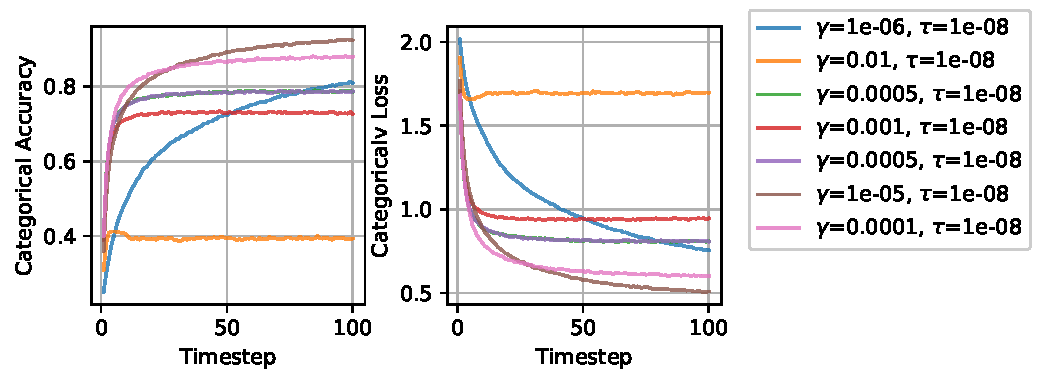
\includegraphics[width=1.\linewidth]{fig/AccuracyLossBNfixedtau.pdf}
        \caption{Fixed $\tau$}
        \label{fig:bnfixedtau}
    \end{subfigure}
    \begin{subfigure}{0.98\textwidth}
        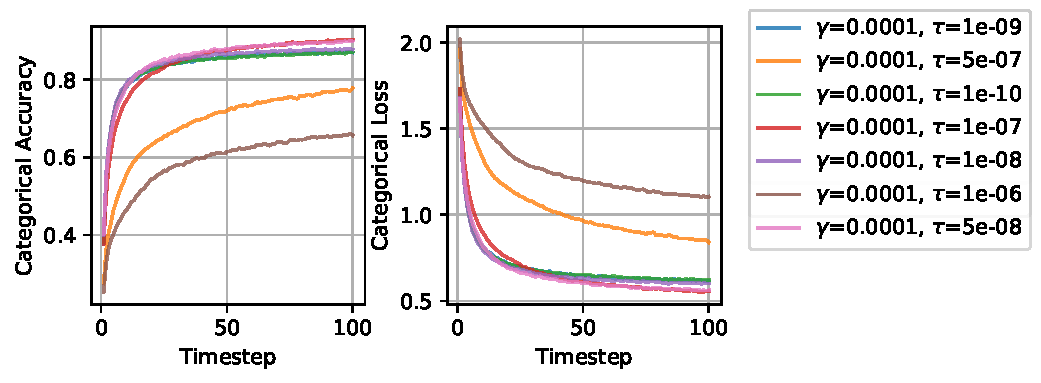
\includegraphics[width=1.\linewidth]{fig/AccuracyLossBNfixedgamma.pdf}
        \caption{Fixed $\gamma$}
        \label{fig:bnfixedgamma}
    \end{subfigure}
    \caption{Ablation studies for $\tau$ and $\gamma$ for Batch Normalization}
\end{figure}

Keeping $\tau$ same ($10^{-8}$) we see the effect of different $\gamma$ in Fig (\ref{fig:bnfixedtau}). From eq (\ref{eqn:gamma}) it is clear that with the increase in the value of $\gamma$, $m_t$ fluctuates more. A high $\gamma (=0.01)$ gives very poor performance as high adaptivity rate makes weight to flip in less time steps if a gradient signal starts pressurizing it. Even though in the very beginning of the training, the accuracy trend is steep in case of $\gamma=0.01$, within a short period of time the accuracy converges to $40\%$. A low $\gamma (=10^{-6})$ provides stable training process but it takes long time to fully converge to final accuracy. From the plots we found for $\tau=10^{-8}$, $\gamma=10^{-5}$ performs best and converges to training accuracy $92.15\%$.

Fig (\ref{fig:bnfixedgamma}) gives training accuracy and loss for different threshold $\tau$ and a fixed $\gamma(=0.0001)$. As explained in the paper, $\tau$ should be a non zero real number but not so big that the weight flipping is hindered. In our simulation result, networks with $\tau$ in the range of $10^{-8}$ perform nearly same. 



\section{Layer Normalization}
Till date in most of the works in the line of BNN, batch normalization is used between consecutive non-linear layers in order to stabilize the training. The aim of batch normalization is to normalize the inputs with the global mean and variance but calculating mean and variance of activations for the whole dataset is very costly. So batch normalization is done in small batches and the estimated mean and variances vary from one minibatch to other. The main challenge of using batch normalization is limitation in batch size.
\begin{figure}[!ht]
    \centering
    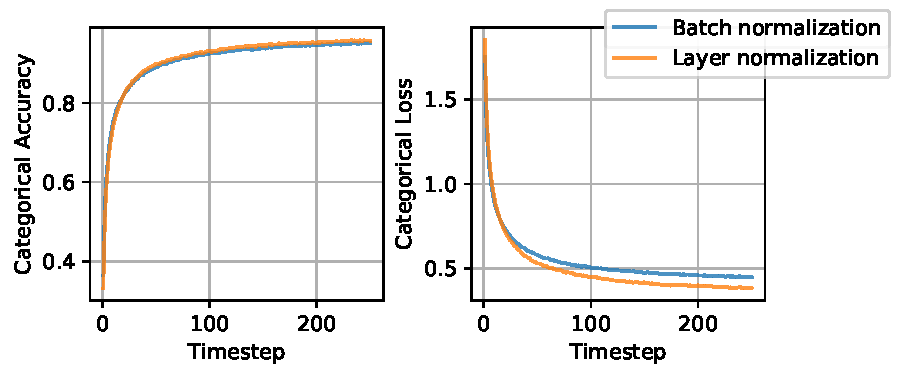
\includegraphics[scale=0.8]{fig/AccuracyLosscompareBNLN.pdf}
    \caption{Comparison of BN and LN with $\tau=10^{-8}$ and $\gamma=10^{-5}$ in Binary VGG net with CIFAR10 dataset and BOP optimizer}
    \label{fig:bnln}
\end{figure}
If the batch size is very small the variance of the estimates would be very high which makes it difficult to use batchnorm in online learning. Also in case of recurrent neural network, use of batchnorm is difficult as the layer statistics change at each timestep. In this section, we look into layer normalization as an alternative solution to avoid these problems \cite{lei2016layer}. 

\begin{figure}[!ht]
\centering
    \begin{subfigure}{0.98\textwidth}
        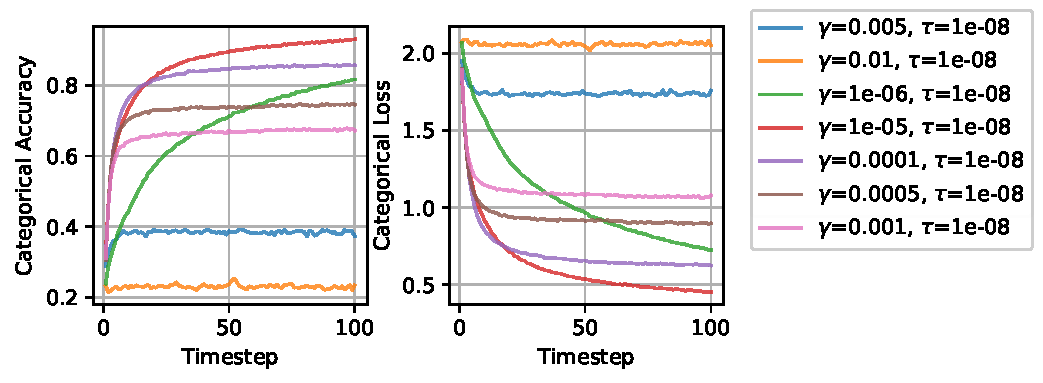
\includegraphics[width=1.\linewidth]{fig/AccuracyLossLNfixedtau.pdf}
        \caption{Fixed $\tau$}
        \label{lnfixedtau}
    \end{subfigure}
    \begin{subfigure}{0.98\textwidth}
        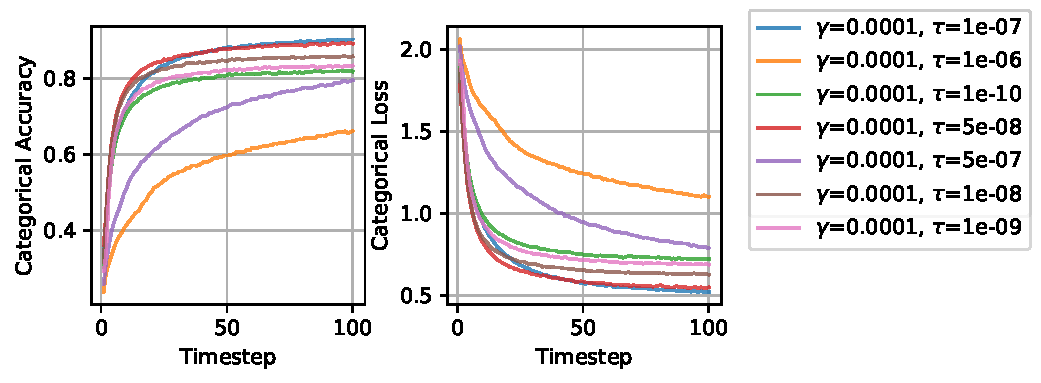
\includegraphics[width=1.\linewidth]{fig/AccuracyLossLNfixedgamma.pdf}
        \caption{Fixed $\gamma$}
        \label{lnfixedgamma}
    \end{subfigure}
    \caption{Ablation studies for $\gamma$ and $\tau$ for layer normalization} \label{fig:ln_ablation}
\end{figure}

Layer normalization works by normalizing across the activation (features) passed between two consecutive layers instead of over a mini batch. In layer normalization, the statistics are calculated across each feature and are independent of other example. We propose to use layer normalization instead of batch normalization as an alternate way of stabilizing training. In Fig \ref{fig:bnln}, we provide a comparison of training performances of layer normalization and batch normalization for $\tau=10^{-8}$ and $\gamma=10^{-5}$. It is clear that layer normalization performs slightly better than batch normalization for this choice of hyper parameter. 


In Fig. \ref{fig:ln_ablation}, we provide a comprehensive ablation study for the effect of hyper parameters of BOP in conjuction with layer normalization. From Fig (\ref{lnfixedtau}), we can observe that for fixed $\tau(=10^{-8})$ the performance of BVGG net is best for $\gamma=10^{-5}$ and the explanation follows from the batch normalization ablation studies. Similarly, as shown in Fig (\ref{lnfixedgamma}) for fixed $\gamma$, $\tau$ in the range of $10^{-8}$ has nearly same performance.

The above studies conclude that layer normalization can be used as a viable alternative to Batch Normalization in the case of training Binary Neural Networks. This can be especially useful in the cases where BNN has to be trained in an online fashion (as in the case of deep reinforcement learning) where acquiring a mini-batch of sufficient size to alleviate the affect of noise variance in estimation is either costly or undesirable.

  
  





    \section{Using BNNs Beyond Classification: Denoising binary Autoencoder}
Most of the works on BNN till date focus on classification tasks as a benchmark for evaluating the performance of BNNs. In this section we explore the usage of BNNs in  denoising auto encoder (AE), called Binary AE, referred as \textit{BAE}. The architecture we consider for this experiment is given in Table \ref{BAE}. Convolution represents 2D convolution layer for AE and quantized 2D convolution layer for BAE. Kernel size of convolution and deconvolution layers is $(3,3)$ and pool size of max pool layers is $(2,2)$ for both AE and BAE. In this AE architecture first three layers make up the encoder and last three the decoder part. At the first layer of the encoder and decoder, real valued inputs are used. STE-sign function is used as activation on current layer inputs for BAE except for the last layer. The last layer is a deconvolution layer with tanh activation. 
\begin{table}[ht]
  \caption{Architecture for Denoising Binary Auto Encoder}
  \label{BAE}
  \centering
  \begin{tabular}{lrcc}
    \hline
    Layer  &  No. of filters & Batch normalization & Activation on input\\
    \midrule
    Convolution + Maxpool &  $32$  & Yes & -  \\
    Convolution + Maxpool &  $16$  & Yes & STE-sign \\
    Convolution + Maxpool &  $8$  & Yes  & STE-sign \\
    Deconvolution + Upsampling2D &  $8$  & Yes  & - \\
    Deconvolution + Upsampling2D &  $16$  & Yes  & STE-sign \\
    Deconvolution + Upsampling2D &  $32$  & Yes  & STE-sign \\
    Deconvolution &  $3$  & Yes & tanh \\
    \bottomrule
  \end{tabular}
\end{table}
Mean square loss is minimized with BOP and a metric called peak signal to noise ratio (PSNR) is calculated to see the performance of the network during training and testing.
\begin{equation}
    PSNR = 10*\log_{10}\left(\frac{max^2}{mse}\right)
\end{equation}
where $max$ is the maximum possible pixel value of the image and $mse$ is the mean square error between original image and the image output from the network. For traditional AE, the architecture is exactly same except that each layer is trained on real weights with relu activation (instead of STE-sign in BAE) except for the last layer. As the architecture of AE is similar to binary AE except few changes, we do not repeat the architecture.
\begin{figure}[!ht]
    \centering
    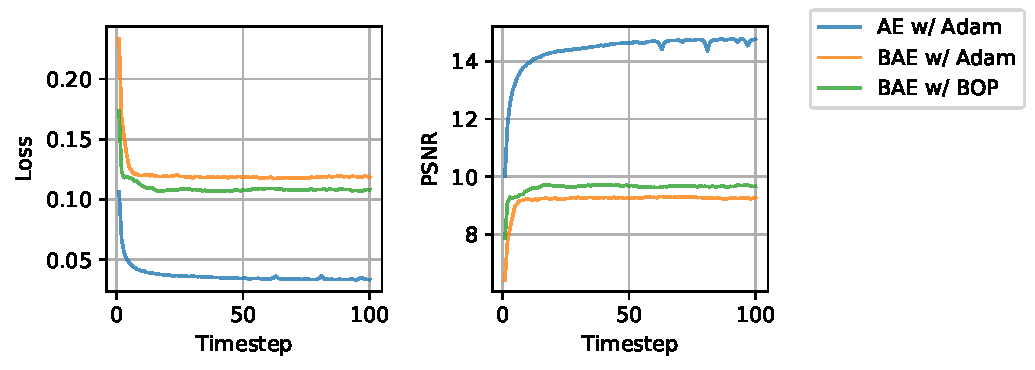
\includegraphics[scale=0.75]{fig/AEtradionalBNNBOP.pdf}
    \caption{Training PSNR (dB); At the end of training, PSNR for AE: $14.76$dB, BAE w/ Adam: $9.25$dB and BAE w/ BOP: $9.66$dB}
    \label{fig:AE}
\end{figure}


\begin{figure}[ht]
\centering
    \begin{subfigure}{0.98\textwidth}
        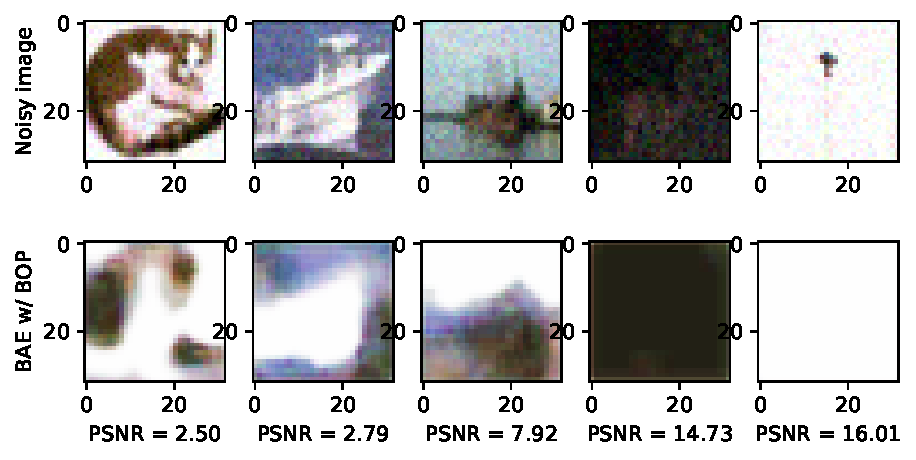
\includegraphics[width=1.\linewidth]{fig/BAEBOPfigsbestworst.pdf}
    \end{subfigure}
    \begin{subfigure}{0.98\textwidth}
        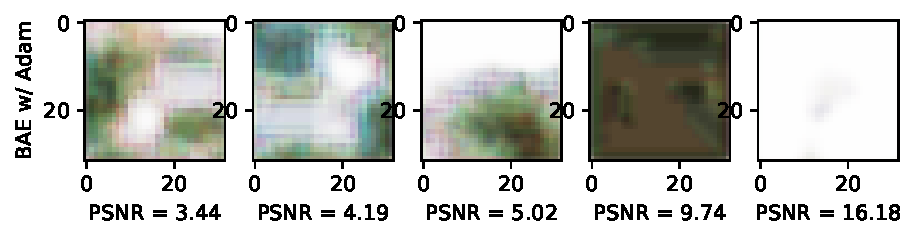
\includegraphics[width=1.\linewidth]{fig/BAEAdamfigsbestworst.pdf}
    \end{subfigure}
    \begin{subfigure}{0.98\textwidth}
        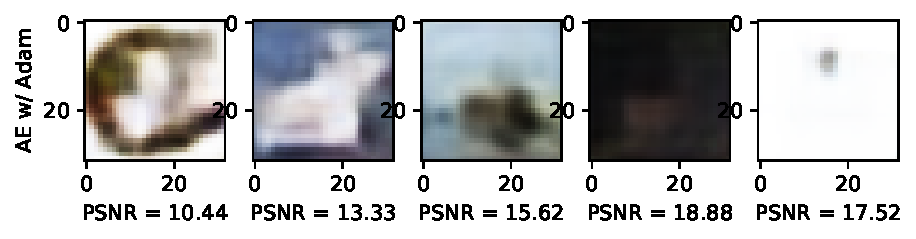
\includegraphics[width=1.\linewidth]{fig/AEAdamfigsbestworst.pdf}
    \end{subfigure}
    \caption{Comparison of recovered images by AE with Adam, BAE with Adam and BAE with BOP}
    \label{fig:AEfig}
\end{figure}

In order to use CIFAR10 dataset for training, we scale the $(32,32)$ images to $(-1,+1)$ say $im_{org}$. The shape of the images are referred as $im_{shape}$. Then a random normal $\mathcal{N}(0,1)$ noise is added with a noise factor $f = 0.1$ and the results are clipped between $(-1,+1)$ again resulting in a noisy image referred as $im_{noi}$.
\begin{equation}
    im_{noi} = \text{clip}\left((im_{org}+f* W), 0, 1\right) \qquad \text{ where } W \sim \mathcal{N}(0,1, im_{shape})
\end{equation}
We perform three sets of experiments, all using batch normalization to stabilize the training with a minibatch size of $64$. The sets are as follows:
\begin{enumerate}
    \item Traditional AE with Adam optimizer (with learning rate $lr = 10^{-3}$, $\beta_1 = 0.99$, $\beta_2 = 0.999$)
    \item BAE with Adam optimizer with same hyper parameters
    \item BAE with BOP optimizer ($\tau=10^{-8}, \gamma=10^{-5}$)
\end{enumerate}
In Fig \ref{fig:AE} the training loss and training PSNR is shown for all three cases. From the graphs we see that, BAE with BOP seems to be better than BAE with Adam for this task and the training converges faster. The test PSNRs of all three cases are as follows:
\begin{enumerate}
    \item AE with Adam: $14.87$ dB
    \item Binary AE with Adam: $9.10$ dB
    \item Binary AE with BOP: $9.30$ dB
\end{enumerate}
However, the results are not impressive for both of the BAE cases. We plot $5$ noisy samples of the CIFAR10 test dataset and the recovered images from the above three cases in Fig. \ref{fig:AEfig}. The reason behind degraded reconstructions for both of the BAE cases are: binary activations cannot pass enough information between the layers to develop a faithful reconstruction. Hence only a reduced finite set of information can be passed between intermediate layers of encoder and decoder. This could be the reason for not so good performance of BAE. We see a huge scope of improvement for BNN in case of BAE as well as other use cases.

    \section{Concluding Remarks}
To summarize our work, we started with studying the effect of using latent weights on BNN. From our observations, it can be concluded that for most of the cases latent weights on BNN do not perform better than binary weights. This conclusion aligns with the authors' claim that binary weight should not be considered as an approximation of latent weights. We also present an ablation study for the choices of two hyper parameters $\tau$ and $\gamma$ for BOP optimizer. Our comprehensive experimental analysis shows the effect of each of these hyper parameters in the optimization procedure. Next, while most of the works only considered batch normalization, we introduce layer normalization as an alternative way of normalization and it shows impressive results. An ablation study on the effects of optimizer hyper parameters shows that layer normalization can provide improved results in some cases. Finally to explore the applicability of BNN in other use cases, we consider Binary AutoEncoders (BAE). The performance of BOP for BAE is then compared with BAE with Adam and AE with Adam. Though a very preliminary results with BAE are shown in our report, BOP shows better PSNR than Adam when used for training binary neural networks.

    \section*{Acknowledgement}
We sincerely thank Code Ocean for the compute support they have provided for this work.
    \bibliographystyle{plainnat}

 	\bibliography{99_library.bib}

\end{document}

